\documentclass[letterpaper, reqno,11pt]{article}
\usepackage[margin=1.0in]{geometry}
\usepackage{color,latexsym,amsmath,amssymb,graphicx, float}
\usepackage{hyperref}

\hypersetup{
colorlinks=true,
linkcolor=magenta,
filecolor=magenta,
urlcolor=cyan,
}

\graphicspath{ {images/} }

\newcommand{\RR}{\mathbb{R}}
\newcommand{\CC}{\mathbb{C}}
\newcommand{\ZZ}{\mathbb{Z}}
\newcommand{\QQ}{\mathbb{Q}}
\newcommand{\NN}{\mathbb{N}}
\newcommand{\st}{\text{ s.t.}\ }
\newcommand{\ep}{\epsilon}

\begin{document}
\pagenumbering{arabic}
\title{PHYS 301 Homework 5}
\date{November 17, 2021}
\author{Xander Naumenko}
\maketitle

{\noindent\bf Question 1a.} The potential is determined by the boundary conditions and Laplace's equation: 

\[
    \frac1X\frac{\partial^2 X}{\partial x^2}+\frac1Y\frac{\partial^2 Y}{\partial y^2}=0    
\]

Since these are each independent they each must be constants of opposite signs, and separating gives the normal solutions to Laplace's equation in Cartesian coordinates. Clearly the $\sin$ component should be for the solution for $Y$, since it's boundary conditions are zero. Therefore we have 

\[
    Y=A\sin(ky)+B\cos(ky)
\]

Applying boundary conditions gives that $B=0$ and $k=\frac{n\pi}{a}, n\in\NN$. For $X$, we have that 

\[
    X=C\sinh(kx)+D\cosh(kx)
\]

Applying the boundary condition on the right gives that $C=0$. For the right side, we must use a fourier series to estimate a step function. The final solution is then in the form 

\[
    V(x, y)=XY=\sum_{n\text{ odd}}A_n\sin(\pi ny/a)\cosh(\pi nx/a)
\]

Using the fourier series derived in the class notes (since this is the exact same boundary condition), we find that 

\[
    A_n=\frac{4V_0}{n\pi\cosh(n\pi)}
\]

\[
    \implies V(x, y)=XY=\sum_{n\text{ odd}}\frac{4V_0}{n\pi\cosh(n\pi)}\sin(\pi ny/a)\cosh(\pi nx/a)
\]

{\noindent\bf Question 1b.} See plots in figures \ref{fig:1bi} and \ref{fig:1bii}. Based on these it can't be a conductor since the electric field lines are not perpendicular to the surface. 

\begin{figure}[htbp]
\centering
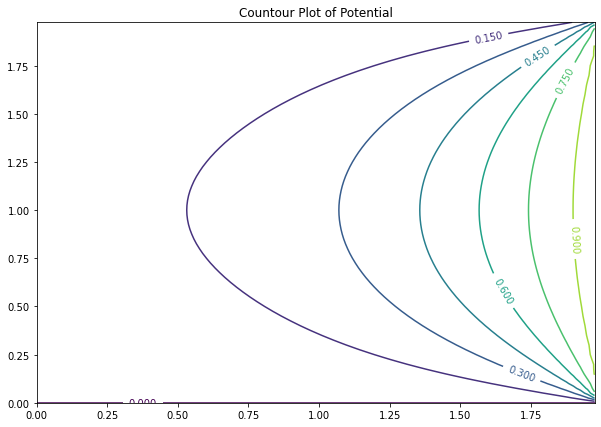
\includegraphics[width=\textwidth]{q1bi}
\caption{Equipotential surfaces for $a=2$ and $V_0=1$}
\label{fig:1bi}
\end{figure}

\begin{figure}[htbp]
\centering
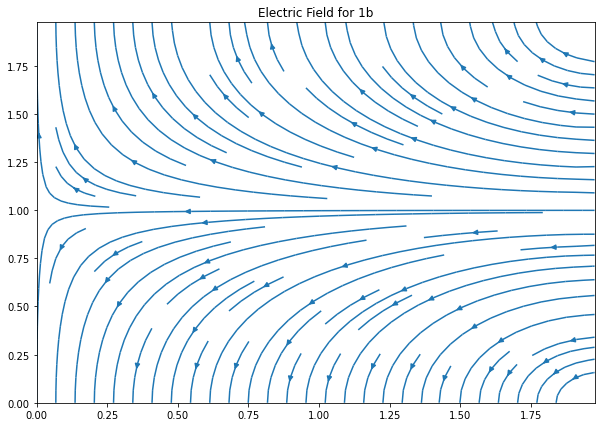
\includegraphics[width=\textwidth]{q1bii}
\caption{Electric field derived from the potential. This was calculated numerically with \texttt{np.gradient()}}
\label{fig:1bii}
\end{figure}

{\noindent\bf Question 1c.} Boundary conditions give that 

\[
    \sigma=-\epsilon_0(E_{out}-E_{in})=\ep_0\frac{dV}{dy}=-\epsilon_0\sum_{n\text{ odd}}\frac{4V_0}{a\cosh(n\pi)}\cosh(\pi nx/a)
\]

% From Gauss's law we know that the Laplacian of $V$ is $-\frac\rho{\ep_0}$. Thus we have 

% \[
%     \rho = -\ep_0\nabla^2 V=-\ep_0\bigg(Y\frac{\partial^2 X}{\partial x^2}+X\frac{\partial^2 Y}{\partial y^2}\bigg)
% \]

% Plugging this in we note that $\frac{\partial^2 Y}{\partial y}=0$ since $Y=\sin(kx)$, so this gives 

% \[
%     \rho = -\epsilon_0\sum_{n\text{ odd}}\frac{4\pi nV_0}{a^2\cosh(n\pi)}\cosh(\pi nx/a)
% \]

{\noindent\bf Question 2a.} Using the double angle formulas we have that $\cos(2\theta)=2\cos^2\theta-1=\frac43(\frac32\cos^2\theta-\frac12)-\frac13=\frac43P_2(\cos\theta)-\frac13P_0(\cos\theta)$. Then because $V$ must obey the laplacian being zero outside, it must be in the form

\[
    V(r, \theta)=\sum_{\ell=0}^\infty(A_\ell r^\ell+B_\ell r^{-(\ell+1)})P_\ell(\cos\theta)
\]

We already know the potential on the outside, and we know the voltage is zero at infinity and finite inside. This means that for inside the sphere, 

\[
    V(r, \theta) = V_0(\frac4{3R^2}r^2(\frac32\cos^2\theta-\frac12)-\frac13)
\]

Outside, it is 

\[
    V(r, \theta) = V_0(\frac4{3r^3}R^3(\frac32\cos^2\theta-\frac12)-\frac R{3r})
\]

{\noindent\bf Question 2b.} Using the boundary conditions of the sphere, we have 

\[
    \sigma=\epsilon_0(E_{out}-E_{in})=\epsilon_0(\frac{dV_{in}}{dr}-\frac{dV_{out}}{dr})=\ep_0V_0(\frac8{3R}P_2+\frac4{R}P_2-\frac1{3R})=\ep_0V_0(\frac{20}{3R}(\frac32\cos^2\theta-\frac12)-\frac1{3R})
\]

{\noindent\bf Question 3.} Assume that the cylinder is oriented along the $z$ coordinates and the applied electric field is along the $x$ axis. Then we have four boundary conditions: $V_{in}(a)=V_{out}(a)$, voltage is finite at the center of the cylinder, $V_{out}(s\to\infty)=-E_0s\cos(\phi)$, and $\frac{\partial V_{out}}{\partial s}=\epsilon_r\frac{\partial V_{in}}{\partial s}$. Since $V$ must fulfill the laplacian in cylindrical coordinates it must be in the form 

\[
    V(s, \theta)=A\log s+B+\sum_{n=1}^\infty (A_ns^n+B_ns^{-n})(C_n\cos(\phi n)+D_n\sin(\phi n))
\]

Using the second and third boundary conditions we know that for outside $A_n=0$ except for $A_1$ and $C_n=D_n=0$ except for $C_1=1$, and for inside $B_n=0$ and A=0. Using the continuity condition gives that 

\[
    V_{in}=B+\sum_{n=1}^\infty A_na^n(C_n\cos(\phi n)+D_n\sin(\phi n))=V_{out}=-E_0s\cos\theta+\sum_{n=1}^\infty B_n a^{-n}C_n\cos(\phi n)
\]

Comparing coefficients this means that $A_n=0$ except for $n=1$. The $E$ field continuity gives 

\[
    \ep_r\frac{\partial V_{in}}{\partial s}=\ep_r A_1\cos\phi=\frac{\partial V_{out}}{\partial s}=-E_0\cos\phi-\frac{B_1}{a^2}\cos\phi
\]

\[
    \ep_r A_1=-E_0-\frac{B_1}{R^2}
\]
\[
    A_1a=\frac{B_1}{a}-E_0 a
\]

\[
    V_{in}=-\frac{E_0}{\ep_r}(1+\frac{\ep_r-1}{\ep_r+1})s\cos\phi
\]

Taking the divergence we get 

\[
    \vec E_{in}=\nabla^2 V=\frac{2E_0}{\ep_r+1}\cos\phi\hat s-\frac{2E_0}{\ep_r+1}\sin\phi\hat\phi=\frac{2E_0}{\ep_r+1}\hat x
\]

{\noindent\bf Question 4.} Setting up a Biot-Savart integral, we get 

\[
    \vec B=\frac{\mu_0}{4\pi}\int_C \frac{Id\ell \times r}{r^3}
\]

For the curved part $d\ell$ and $r$ are perpendicular, whereas for the flat part they are misaligned an angle. Also note that the two flat parts both contribute equally to the $B$ field. Altogether we get that 

\[
    B=\hat z\frac{\mu_0I}{4\pi}\bigg(2\int_{-\infty}^0\frac{Rdx}{(x^2+R^2)^{3/2}}+\int_0^{\pi/2}\frac R{R^2}d\theta\bigg)=\hat z\frac{\mu_0I}{4\pi}\bigg(\frac{2x}{R\sqrt{x^2+R^2}}\bigg|_{-\infty}^0+\frac\pi{2R}\bigg)
\]

\[
    =\frac{\mu_0I}{4\pi}(\frac2R+\frac\pi{2R})\hat z
\]

{\noindent\bf Question 5a.} First, note that the $B$ field must be purely in the $\hat y$ direction. To see why think about strips of current along the $x$ axis and very thin in the $y$ direction. Then each strip is like a thin wire of current, with each contributing nothing the the $\hat z$ direction and by symmetry the net effect on the $B$ field is zero in the $\hat x$ direction. Next consider the Amperian rectangular loop of width w and heigh h with surface normal parallel to the surface current. Then applying Ampere's law, we get 

\[
    \mu_0I_{enc}=\oint_C\vec B\cdot\vec dl\implies w\mu_0K_0=\pm2B(h/2)w\implies B(z)=\begin{cases}-\frac{\mu_0K_0}{2}\hat y&\text{ if }z>0\\\frac{\mu_0K_0}{2}\hat y&\text{ if }z<0\end{cases}
\]

{\noindent\bf Question 5b.} By superposition, the fields of the two add. Thus in between it is just twice what the field would be with just one, and in inside and outside the field cancels to zero. 


\[
    \mu_0I_{enc}=\oint_C\vec B\cdot\vec dl\implies w\mu_0K_0=\pm2B(h/2)w\implies B(z)=\begin{cases}-\mu_0K_0\hat y&\text{ between }\\0&\text{ above and below }\end{cases}
\]

{\noindent\bf Question 5c.} Consider the same Amperian loop as in part a. Then we get that for the top, 

\[
    \mu_0I_{enc}=\int_0^w\int_{-h/2}^{h/2}J_0|z|dz dy=\frac{w\mu_0J_0h^2}4=\oint_C\vec B\cdot\vec dl=-2B(h/2)w
\]

\[
    \implies B_{inside, above}(z)=-\frac{\mu_0J_0z^2}{2}
\]

By symmetry the bottom of the slab is 

\[
    \implies B_{inside, below}(z)=\frac{\mu_0J_0z^2}{2}
\]

Using the exact same process except now with the the Amperian loop now outside as well gives 

\[
    \implies B_{outside, above}(z)=-\frac{\mu_0J_0h^2}{2}
\]


\[
    \implies B_{outside, below}(z)=-\frac{\mu_0J_0h^2}{2}
\]

\end{document}